\documentclass{article}%
\usepackage[T1]{fontenc}%
\usepackage[utf8]{inputenc}%
\usepackage{lmodern}%
\usepackage{textcomp}%
\usepackage{lastpage}%
\usepackage[head=40pt,margin=0.5in,bottom=0.6in]{geometry}%
\usepackage{graphicx}%
%
\title{\textbf{Vecinos de Colinas del Neverí protestaron por falta de agua y aseo urbano}}%
\author{El Nacional Web}%
\date{28/09/2018}%
%
\begin{document}%
\normalsize%
\maketitle%
\textbf{URL: }%
http://www.el{-}nacional.com/noticias/protestas/vecinos{-}colinas{-}del{-}neveri{-}protestaron{-}por{-}falta{-}agua{-}aseo{-}urbano\_253564\newline%
%
\textbf{Periodico: }%
EN, %
ID: %
253564, %
Seccion: %
Protestas\newline%
%
\textbf{Palabras Claves: }%
Anzoátegui, Protestas, Sociedad\newline%
%
\textbf{Derecho: }%
2.8, %
Otros Derechos: %
, %
Sub Derechos: %
2.8.1\newline%
%
\textbf{EP: }%
SI\newline%
\newline%
%
\textbf{\textit{Los residentes trancaron la Intercomunal para exigir respuesta por parte del organismo correspondiente ~}}%
\newline%
\newline%
%
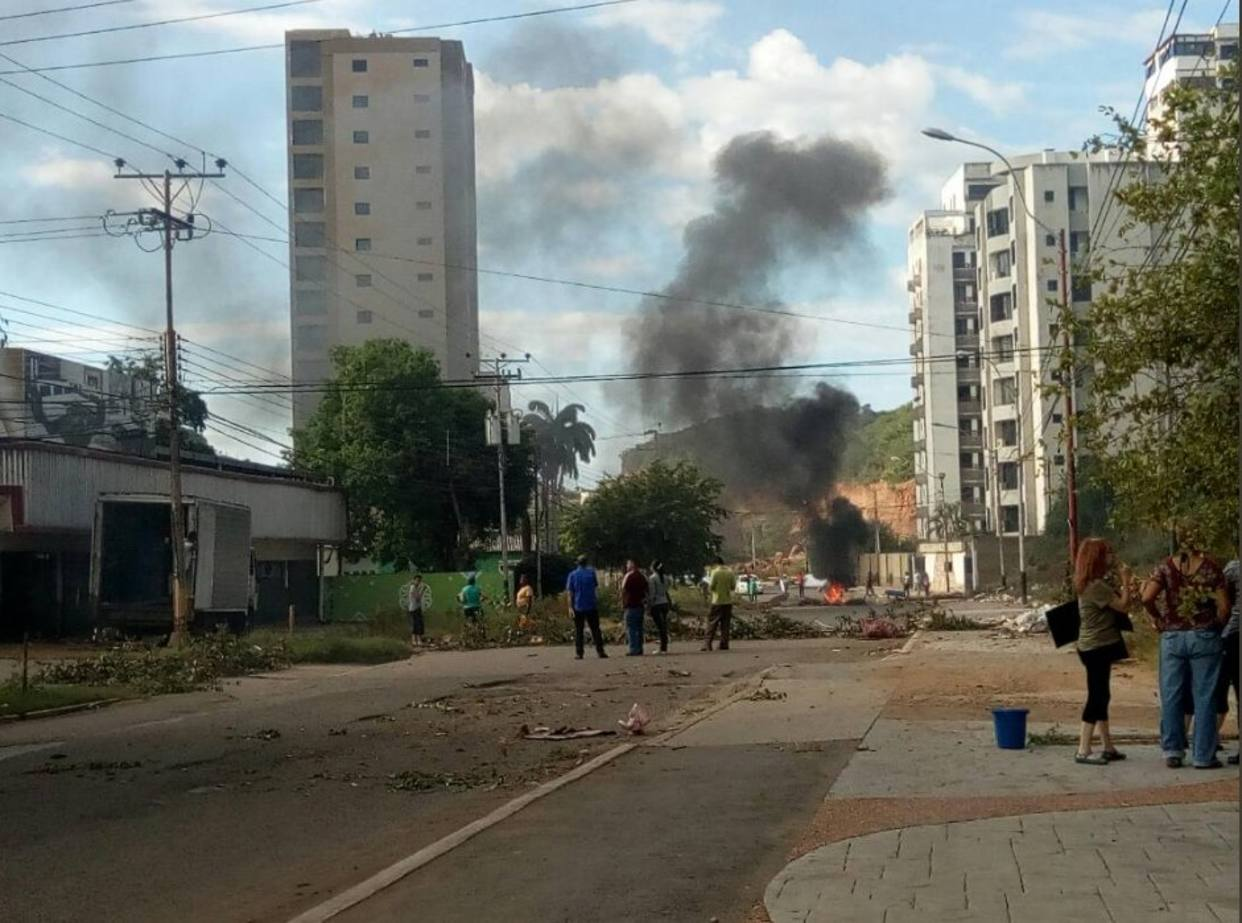
\includegraphics[width=300px]{154.jpg}%
\newline%
%
Habitantes del sector Colinas del Neverí en el municipio Bolívar, estado Anzoátegui, protestaron~desde horas de la mañana en la zona por falta de servicios básicos.%
\newline%
%
Los ciudadanos denunciaron que tienen un mes sin agua y dos meses sin aseo urbano. Usuarios en las redes sociales informaron que son más de 500 familias que tienen 31 días sin el servicio.%
\newline%
%
Los habitantes agregaron que no abrirán el paso vehicular hasta obtener una repuesta por parte de Hidrocaribe.%
\newline%
%
\end{document}